\documentclass{article}
\usepackage[letterpaper, total={7in, 8in}]{geometry}
\usepackage[utf8]{inputenc}
%\usepackage[english]{babel}
\usepackage[]{amsthm} %lets us use \begin{proof}
\usepackage[]{amsmath}
\usepackage[]{amssymb} %gives us the character \varnothing
\usepackage{mathrsfs}
\usepackage{graphicx}
\usepackage{adjustbox}
\usepackage{titlesec}
\usepackage[numbered,framed]{matlab-prettifier}
\usepackage{listings}
\usepackage[t1,OT1]{fontenc}
\usepackage{filecontents}
\usepackage{float}
\usepackage{physics}
\usepackage{csvsimple}
\usepackage{booktabs}
\usepackage{longtable}
\usepackage{algorithmicx}
\usepackage{mathtools}
\usepackage{breqn}
\usepackage{framed,color}
\usepackage{amsmath,mleftright}
\usepackage{xparse}
\usepackage{titling}
\usepackage{tabularx}

\usepackage{hyperref}

\setlength{\droptitle}{-10em}   % This is your set screw

\NewDocumentCommand{\evalat}{sO{\big}mm}{%
	\IfBooleanTF{#1}
	{\mleft. #3 \mright|_{#4}}
	{#3#2|_{#4}}%
}


\DeclareMathOperator{\atantwo}{atan2}

\titleformat{\section}{\normalfont\Large\bfseries}{Section \thesection.}{1em}{}
\titleformat{\subsection}{\normalfont\bfseries}{\alph{subsection})}{1em}{}
%\definecolor{shadecolor}{gray}{0.9}

\title{Smart Products Lab 3}
\author{Tyler Morrison}
\date\today

%\lstset{
%	style              = Matlab-editor,
%	basicstyle         = \mlttfamily,
%	escapechar         = ",
%	mlshowsectionrules = true,
%	literate = {-}{-}1, % <hyphens will not show up unless you add this
%}

\lstset{
	language=C++,
	basicstyle=\ttfamily,
	keywordstyle=\color{blue}\ttfamily,
	stringstyle=\color{red}\ttfamily,
	commentstyle=\color{green}\ttfamily,
	morecomment=[l][\color{magenta}]{\#},
	numbers=left,
	stepnumber=1,
	frame=single
}

\renewcommand{\lstlistingname}{Program}% Listing -> Algorithm

\begin{document}
\maketitle
\section{}
\subsection{Prelab Step 1}
%Clock frequency
The clock frequency is 100 kHz.
%Time constant rising data
With 1 k$\Omega$ pull-up resistors, the time constant, as determined by an exponential fit to the rising data line is, $3.35 \times 10^{-8}$ seconds.
%Time constant falling data
The falling line has significant undershoot which means it has second-order behavior. As such, it is difficult to identify an exact time constant from the output because it is either an underdamped second order system or a system with two dominant poles on the real axis that are near to each other. Considering these possibilities, I estimate a time constant of around $7 \times 10^{-8}$ to $1 \times 10^{-7}$ seconds.
%OVershoot rising/falling
Undershoot on this falling data line was about 23 percent of the difference between the high and low logic levels on the data line.
\subsection{Prelab Step 2}%0.1uF calacitor
%Time constaant falling or rising. Program output
Adding the 0.1$\mu$F capacitor increased the rising data time constant to $7.25 \times 10^{-5}$ seconds and increased the falling data time constant to $6.46 \times 10^{-6}$ seconds and as a result, the Pi failed to communicate with the device at all.
%Other resistance/capacitors
Adding a 1k$\Omega$ resistor in series with the capacitor was enough to drop the falling time constant back down to about $1.7 \times 10^{-8}$ seconds and permit communication to occur again.
\begin{figure}[H]
	\centering
	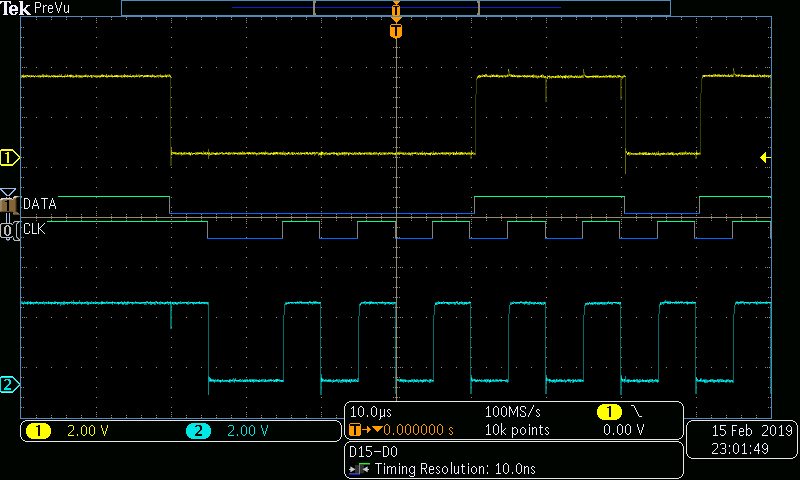
\includegraphics[keepaspectratio,width=.6\linewidth]{./prelab_screenshots/1.png}
	\caption{I2C clock and data lines with 1k pull-up resistor.}
\end{figure}
\begin{figure}[H]
	\centering
	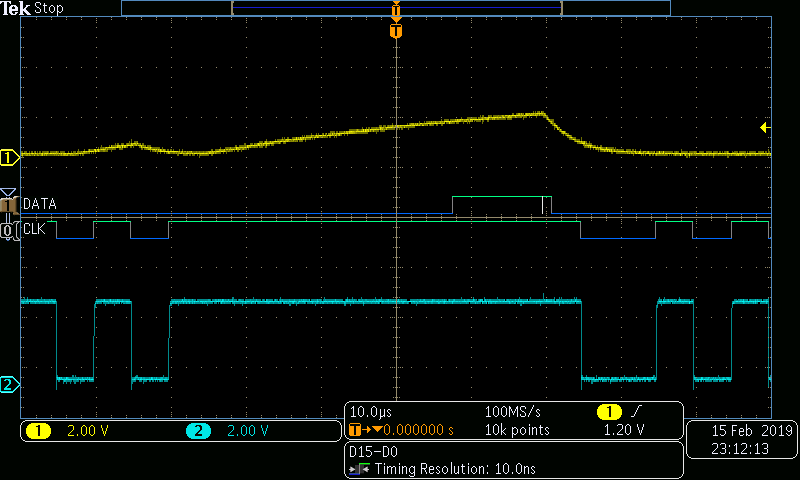
\includegraphics[keepaspectratio,width=.6\linewidth]{./prelab_screenshots/2.png}
	\caption{I2C clock and data lines with 1k pull-up resistor, and 1uF capacitor.}
\end{figure}
\begin{figure}[H]
	\centering
	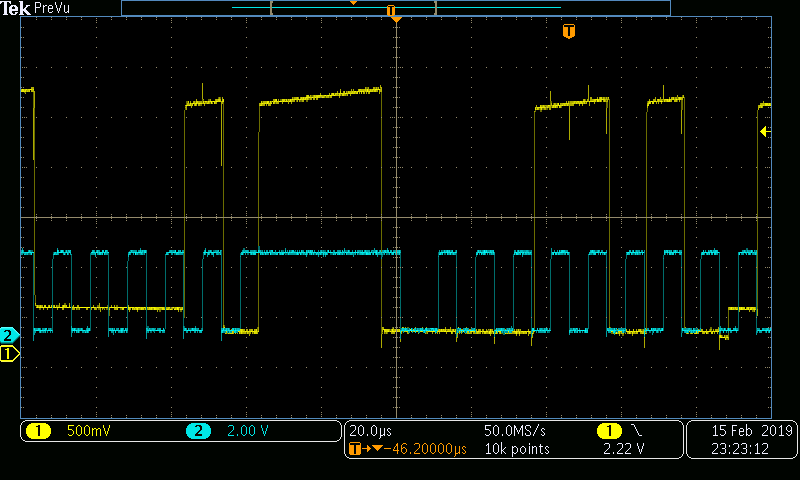
\includegraphics[keepaspectratio,width=.6\linewidth]{./prelab_screenshots/3.png}
	\caption{I2C clock and data lines with 1k pull-up resistor, and 1uF capacitor in series with 1k resistor.}
\end{figure}
\section{}
\subsection{Solution Implementation}
I intentionally used fewer classes than the example. I wanted one class for each chip. For what we have to do in this lab, I did not feel the need to write a whole other class to wrap the two together. If we end up using this setup more in the future to the extent that I feel the need to simplify random reading and writing across multiple EEPROMs via the multiplexer, that will be a very very simple addition.
\begin{itemize}
	\item \texttt{class MC24XX} in \texttt{24XXEEPROM.h}
		\begin{itemize}
			\item \texttt{void write(int add, int data)}: writes data byte to address using \texttt{wiringPiI2C}. Sleeps thread for 4000 microseconds to permit complete writing.
			\item \texttt{int read(int add)}: reads data bye to address using \texttt{wiringPiI2C}.
			\item \texttt{MC24XX()}: constructor runs the Wiring Pi I2C setup setting slave.
		\end{itemize}
	\item \texttt{class CD405} in \texttt{CD405PLEX.h}
		\begin{itemize}
			\item \texttt{CD405(int pinA, int pinB)}: constructor declares the two pins that control the multiplexer. 
			\item \texttt{void setPlex(int c)}: sets the multiplexer switch to the given mode 0-3.
		\end{itemize}
	\item Typical use switching EEPROMs and writing to an address.
\end{itemize}
\begin{lstlisting}
cd405.setPlex(i); // Switch to multiplexer i
mc24xx.write(j, data[j]); // Write to register address j, data element j
\end{lstlisting}
\subsection{Read/Write Timing}
I tested timing required for reads and writes by running and compiling my test script while decreasing the wait times for read and write until errors occurs. Testing on my Pi, I got down to 4000 microsecond waits for writes and no waiting for reads. Without waiting on writes, the write had undefined behavior when checked with a subsequent read. Sometimes it seemed to be the previously written value. Sometimes I couldn't explain the value written and subsequently read back. No wait was need in the read, perhaps because the thread knows it has to wait to read in the value required before continuing execution. Perhaps there exists some way to implement this same concept for writes that eliminates the need for open loop waits. In any case, write speed is much slower.

\subsection{Incremental Testing}
I utilized incremental testing by first practicing switching the multiplexer with LEDs indicating success, then wrapping this code in a class, then adding in the EEPROM and finally be implementing a full random data read/writes test across all registers and EEPROMs with error checking.

\section{}
\subsection{Measurements and screenshots}
%Pull-up resistor
The pull-up resistor we used was 2k$\Omega$.
%Clock frequency
The clock frequency was 100kHz.
%Rise time for rising edge data
The 10\% to 90\% rise time for the rising edge of the data line at the EEPROM was about $2.30 \times 10^{-7}$ seconds or about 230 ns.
%Rising/falling overshoot
There was no overshoot on the rising line. There was undershoot of about 11\% of the logic high to logic low difference on the falling edge at the output pin of the Pi, however by the time the signal propagated to the input pin of the EEPROM, there was no undershoot. This is not surprising considering the additional damping discovered in the EEPROM.
%Screenshot of digital/analog signals
\begin{figure}[H]
	\centering
	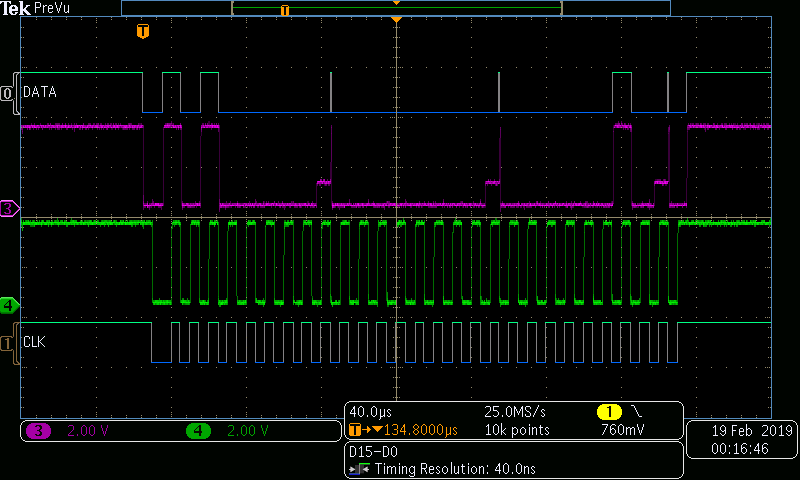
\includegraphics[keepaspectratio,width=.6\linewidth]{./lab_screenshots/tek00001.png}
	\caption{These are the analog and digital bus signals for the data and clock lines at the Pi. The signal includes a write command to the EEPROM with address 0x50, the register address 0x0, and the data value 0x2 which can all be clearly seen and verify the i2c implementation.}
\end{figure}

\subsection{Signal timing across multiplexer}
The signal falling from logic high to about 0.5 V had about a $1.68 \times 10^{-8}$ second delay from the Pi side of the multiplexer to the EEPROM side of the multiplexer - and was remarkably consistent across all multiplexer channels. This delay was not a transport delay but rather the delay associated with increasing the time constant of the circuit node on the EEPROM side of the multiplexer - likely as the result of extra parasitic capacitance in the multiplexer.

\section{}
I wrote my own code for the lab.cpp file to fully test the EEPROM-multiplexer setup. Here is a portion of the output of my test for lab four.
\lstset{
	language={},
	basicstyle=\ttfamily,
	keywordstyle=\color{blue}\ttfamily,
	stringstyle=\color{red}\ttfamily,
	commentstyle=\color{green}\ttfamily,
	morecomment=[l][\color{magenta}]{\#},
	numbers=left,
	stepnumber=1,
	frame=single
}

\lstinputlisting[caption = {Output of labthree.cpp},firstline=776,firstnumber=776,lastline=777]{../lin/main.sol}

Here we can see that I2C is PAINFULLY slow and why we only use it for simple components, small data, and not for actual computing.
\end{document}